\chapter{Příklady virtualizace síťových funkcí}

V této kapitole budeno několik příkladů, jak lze jednoduše vytvořit NFV v prostředí OpenStack a OpenContrail pomocí heat templatu. Všechna uvedená řešení byla testována v 


\begin{figure}[h]
\begin{centering}
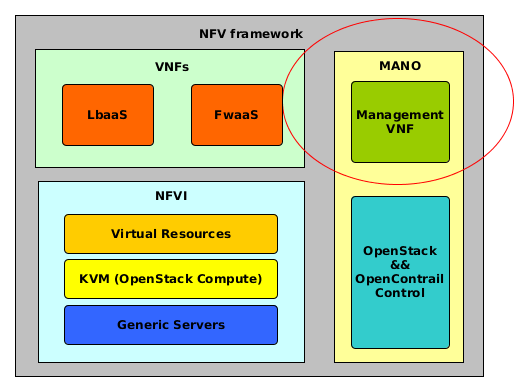
\includegraphics[scale=0.21]{images/VNF_overview}
\par\end{centering}
\caption{Architektura řešení\label{fig:VNF_overview}}
\end{figure}


\section{LbaaS}\label{sub:interaction}

Load-balancer as a Service má umožňovat uživatelům jednoduše 

\subsection{Neutron HAproxy}\label{sub:interaction}


\subsection{AVI networks}\label{sub:interaction}


\section{FwaaS}\label{sub:interaction}



\subsection{PfSense}\label{sub:interaction}

PFSense je open-source firewall/router postavený nad operačním systémem FreeBSD.

\subsection{Fortigate VM}\label{sub:interaction}



